\chapter{Dataset Framework, Exploration and Analysis}
\label{cha:dataset}

This chapter has two purposes: firstly, to detail a programmatic framework developed in order to generate data and to engineer it for machine learning model purposes; and secondly, to explore the data space using visualisation and statistical techniques.

\section{Framework}

This section details the programmatic framework \cite{Jones2018} developed during this PhD. This framework was produced in order to streamline the development and optimisation of surrogate machine learning model for this project. The framework is provided free and open source with the intention that other researchers will adapt and use it for their own surrogate machine learning purposes. Using this repository, the accompanying dataset \cite{huw_rhys_jones_2022_6967536} and the attached guide, the method and results presented in this thesis can be reproduced by anyone.
\\

\noindent
The framework is developed so as to be useable on a portable batch system (PBS) as is commonly implemented on university cluster computing systems. These systems allow job queuing and parallel processing of experiments \cite{henderson1995job}. If a PBS system is not available, the framework is functional on any other standard computer.
\\

\noindent
The framework has three principal functions:

\begin{enumerate}
	\item The creation of Parmec data 
	\item The extraction of relevant data from Parmec data cases
	\item The translation and engineering of the aforementioned data in datasets useable as machine learning training data 
\end{enumerate}

\subsection{Parmec Data Generation}

The Parmec case generation tool allows batch generation of instances, each traceable to a pseudo-random number seed \cite{blum1982simple}. This allows a creation of a large and reproducible dataset. Should the dataset be lost/corrupted or need to be temporarily deleted, it can be exactly reproduced using the original seeds.
\\

\noindent
This tool was developed by adapting an industry standard Microsoft Excel sheet with extensive changes using the Visual Basic .NET framework \cite{grundgeiger2018programming}. Using this tool, the user can batch generate Parmec configuration files. 
\\

\noindent
For ease of use and interaction by the user, the framework converts each Parmec case into a data object, making use the object oriented programming (OOP) paradigm \cite{meyer1997object} with the Python language \cite{deitel2002python}. The Parmec class has interface methods which allow simple access and parsing of the information about that case. An additional layer of abstraction is provided by the creation of additional classes which aggregate all of the Parmec case objects in a batch of cases. This allows then generation of datasets for use in visual analysis or machine learning.
\\

\noindent
Using the aforementioned tool, 8300 Parmec examples were generated to form the base dataset. Approximately 75\% of the dataset was randomly partitioned to become the training set (N) with around 6300 instances, with the remaining 25\% (2000 samples) forming the test set ($N_t$). The full list of inputs and outputs to the Parmec model are summarised in Table~\ref{tab:parmecIO}.
 

\subsection{Model Inputs (Features)}

 Fuel bricks are stacked in a multi-level structure as mentioned in section~\ref{AGR}. There are 7 levels (l~=~7), each with 284 bricks (f~=~284), hence there are 1988 fuel bricks in the reactor in total (r~=~1988). The input configuration files contain a integer representation of the cracking status of each brick in the core as visualised in Figure~\ref{fig:cascade}. In the aforementioned figure, an uncracked brick is represented by a -1, with cracked bricks represented by an integer 1 - 4, with this number giving the orientation (see Figure~\ref{fig:orientations}). Note that each core level has 18 rows and columns (d~=~18) but not every element represents a fuel brick - corner positions are padded with zeros.
 \\
 
\begin{figure}[t]
	\centering
	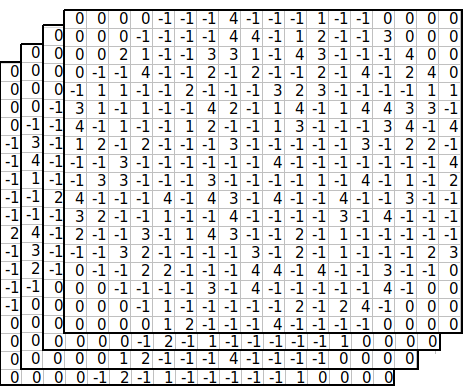
\includegraphics[scale=0.45]{Figures/InputCascade.png}
	\caption{Multi-channel Cascade}
	\label{fig:cascade}
\end{figure}

\begin{figure}[t]
	\centering
	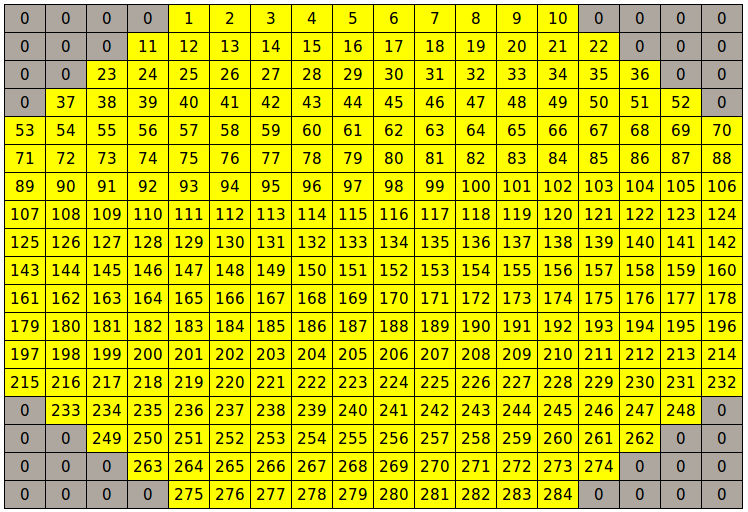
\includegraphics[scale=0.35]{Figures/fuel_channel_numbers.png}
	\caption{Fuel Brick Encoding Order}
	\label{fig:order}
\end{figure}


\noindent
With 6300 training samples and 1988 input parameters (cracked or uncracked AGR bricks) this gives a matrix of dimensions N by BF (6300 x 1988), hence our feature matrix is defined as $\textbf{X} = \{-1, 1\}^{N \times BF}$. This matrix serves as the base input features to the machine learning models described in the following section. The cracking status of all fuel bricks are encoded according to their level (bottom to top) then by their position as shown in Figure~\ref{fig:order}.
\\

\noindent
The aforementioned data framework which includes the Parmec case class allows the user to access input information about a particular case.  For example, should the user want to get the number of cracks in a particular level of the core. Used in aggregate across all cases within the dataset, the above input feature matrix as described in the previous paragraph can be efficiently obtained. 
 

\subsection{Model Outputs (Labels)}


Recall from subsection~\ref{Engineering} that the Parmec model is used to simulate an earthquake (Figure~\ref{fig:earthquake}). This includes a settle down period before and after the earthquake proper. For 271 regular time intervals (TI) throughout the earthquake simulation, the model outputs a data-file. This file contains translation and rotation data for all bricks within the reactor core. 
\\

\noindent
There are 4173 interstitial bricks (henceforth referred to by the notation BI), the behaviour of which we are interested in during the earthquake time history. Like the fuel bricks discussed in the previous subsection, the interstitial bricks are stacked into levels. As the interstitials are shorter than their fuel equivalent, an interstitial channel is made of a stack of 13 bricks. Similar to the encoding process for fuel bricks, interstitials are encoded in order of their level and then by the order as given in Figure~\ref{fig:inter_order}.
\\

\noindent
For each interstitial brick, Parmec calculates 6 output metrics (OM) representing displacement in and rotation about all three Cartesian directions. With the 271 time intervals mentioned above, this results in nearly 6.8 million outputs per Parmec case. Therefore, each Parmec case has an output as can be represented by (\ref{instance_result_matrix}) with each value being normalised element-wise across the entire dataset.  
\\

\begin{figure}[t]
	\centering
	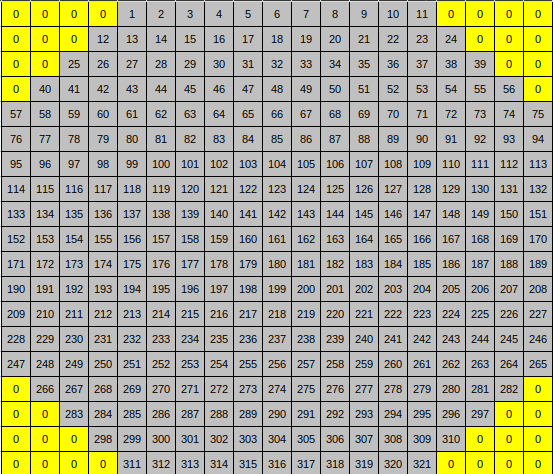
\includegraphics[scale=0.35]{Figures/inter_channel_numbers.png}
	\caption{Interstitial Brick Encoding Order}
	\label{fig:inter_order}
\end{figure}

\noindent


\begin{equation} \label{instance_result_matrix}
	Y_i = \{0, 1\}^{BI \ \times \ TI \ \times \ OM}
\end{equation}

\begin{table}[h!]
	   \begin{center}
		
		\begin{tabular}{c|c|c|r|c} % <-- Alignments: 1st column left, 2nd middle and 3rd right, with vertical lines in between
			\textbf{Inputs} & \textbf{Outputs}  \\
			
			\hline
			& \\
			\textbf{Cracking Status}   &  \textbf{ Brick Displacement} \\
			1988 Fuel Bricks:         & 4173 Interstitial Bricks: \\ 
			7 levels    & 13 levels       \\
			284 fuel bricks per level &  321 bricks per level  \\
			&    \\
			& \textbf{Output Metrics}  \\
			& 6 per interstitial brick: \\ 
			
			&  3 translational \\
			&  3 rotational \\
			
			& \\
			
			\textbf{Earthquake Acceleration} & \textbf{Output Frequency} \\
			1400 time points: &              271 output points:     \\
			14 seconds &  once per 0.05 seconds    \\
			100 time points per second &     \\
			
			& \\
			
			Fuel brick cracking & Output for all \\
			status is constant & 4173 interstitial bricks \\
			throughout earthquake & and 6 output metrics \\
			& per time point \\
			
			
		\end{tabular}
		\caption{Summary of the Inputs and Outputs of the Parmec Engineering Model for AGR Graphite Core Seismic Analysis.}
		\label{tab:parmecIO}
		   \end{center}
\end{table}


\begin{figure}[ht]
	\centering
	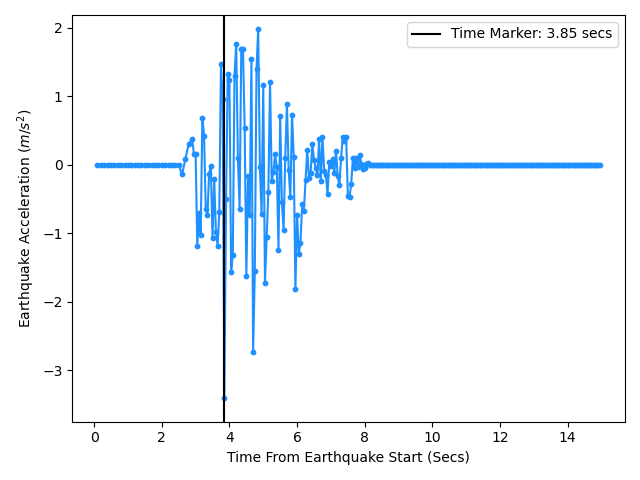
\includegraphics[scale=0.35]{Figures/earthquake.png}
	\caption{History of Acceleration During a Severe Earthquake. Note the settling period before and after the earthquake proper. The true earthquake history includes an acceleration value every 100th of a second. This plot shows a sample every 10th of a second, which is the interval that the Parmec model outputs displacement data. Also shown is a vertical marker, indicating the selected time frame.}
	\label{fig:earthquake}
\end{figure}

\noindent
The large amount of output data generated by Parmec is not in a format readily accessible or interpretable by human users or by other computer analysis. Therefore, the Parmec class object was extended to analyse this data and produce useable outputs. Again, this data is accessible via interactive Parmec object method calls and can be used in aggregate across the entire dataset.


\section{Dataset Exploration and Analysis}

To help choose a direction for research, a visual inspection of the data-set has been made. As mentioned in the previous section, the data produced by the Parmec model is multidimensional. Therefore, visual analysis will be made from multiple perspectives.

\subsubsection{Time History: Example Cases}


For a chosen case, Figures~\ref{fig:time_history_1} and \ref{fig:time_history_2} show the displacement time history for selected channels in two directions. It can be seen that the oscillations in displacement largely follow those of the earthquake acceleration pattern (Figure~\ref{fig:earthquake}). As expected, there is no displacement during the preliminary settle down period up to about 2.5 seconds. Channels near the centre of the core see higher amplitudes, with some of the most central channels also continuing to move after the earthquake has ended at ~8 seconds.  
Selecting four time frames from the earthquake time history, it is possible to visualise the displacement in the reactor core at these points. The time frames chosen can be seen in Figure~\ref{fig:earthquake} with vertical indicators and were chosen as they represent the peaks of earthquake acceleration. 
\\

\begin{figure*}[p]
	\centering
	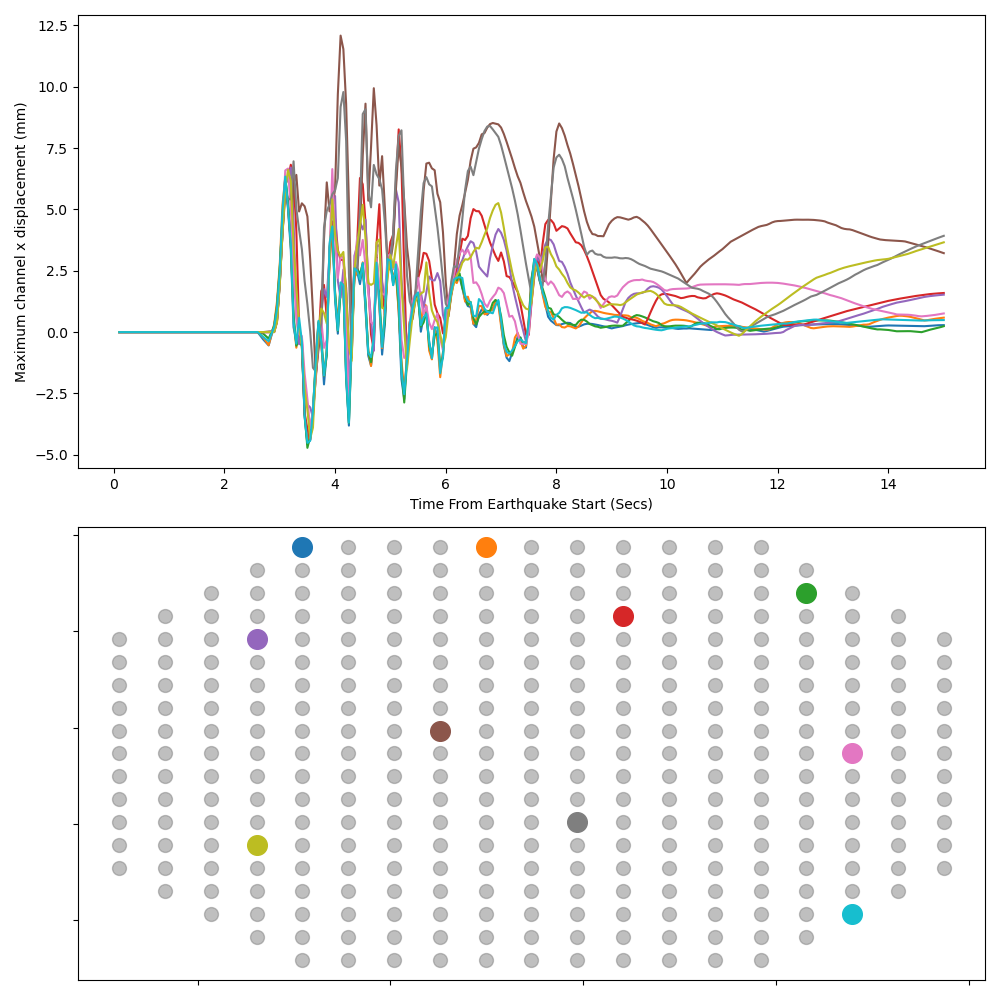
\includegraphics[scale=0.45]{Figures/time_history.png}
	\caption{Time History: Maximum Channel Displacement in the West to East Direction for Sample Channels. Compare with the earthquake time history (Figure~\ref{fig:earthquake}).}
	\label{fig:time_history_1}
\end{figure*}

\begin{figure*}[p]
	\centering
	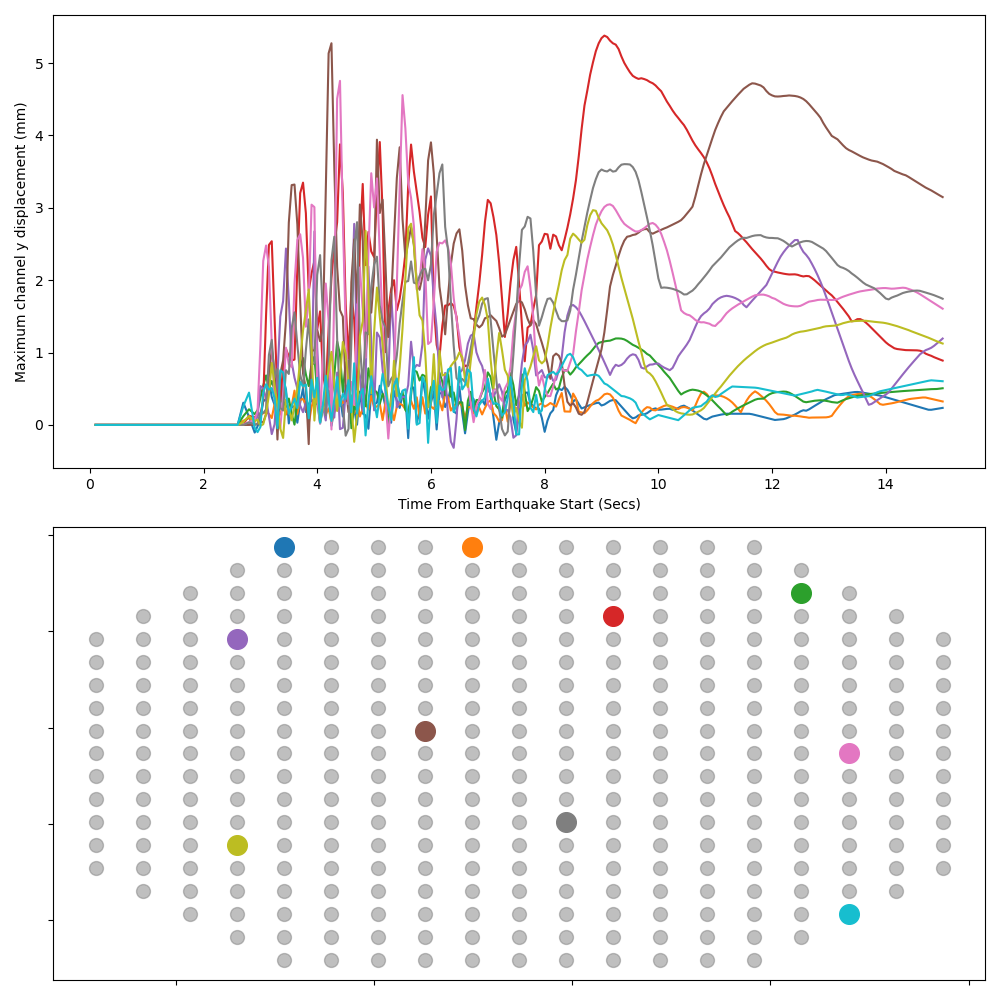
\includegraphics[scale=0.45]{Figures/time_history_y.png}
	\caption{Time History: Maximum Channel Displacement in the South to North Direction for Sample Channels. Compare with the earthquake time history (Figure~\ref{fig:earthquake}).}
	\label{fig:time_history_2}
\end{figure*}

\noindent
A top down view of channel displacements can be seen in Figures~\ref{fig:results1}
and \ref{fig:results2}, where displacements in the west-east and south-north direction can be seen, respectively. For west-east displacement (Figure~\ref{fig:results1}), note that those channels near the edge of the core tend to displace in the opposite direction to those in the centre. For frames 65 and 68, there seems to be little diversity in the distribution of displacement values, whereas for frames 48 and 55 there is more variation, at least for the more central channels. For south-north displacements (Figure~\ref{fig:results2}) the displacements for each case are a variation on a similar pattern in each time frame.
\\

\begin{figure*}[p]
	\centering
	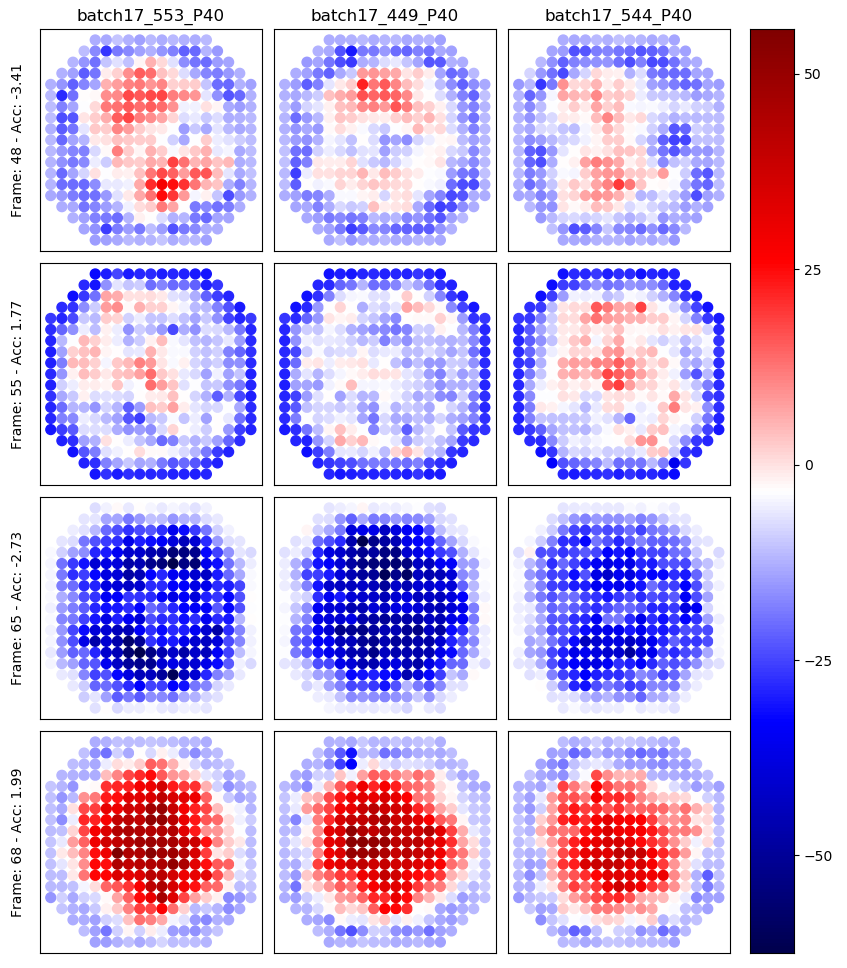
\includegraphics[scale=0.45]{Figures/results1.png}
	\caption{Comparing the Output of Three Cases Through Time: Sum of Channel Displacement in West-East Direction (mm). Three cases have been chosen at random from the data-set, corresponding to each of the three columns in this Figure. Each row corresponds to a time index of the earthquake (see the vertical markers in Figure~\ref{fig:earthquake}). The time frame is listed, as well as the earthquake acceleration at that time. The images are a graphical representation of the displacement value for each interstitial channel. Note that values are in the range $ \pm 50 $ i.e. the overall movement of that channel may be up to 50 mm in the left or right direction.}
	\label{fig:results1}
\end{figure*}

\begin{figure*}[p]
	\centering
	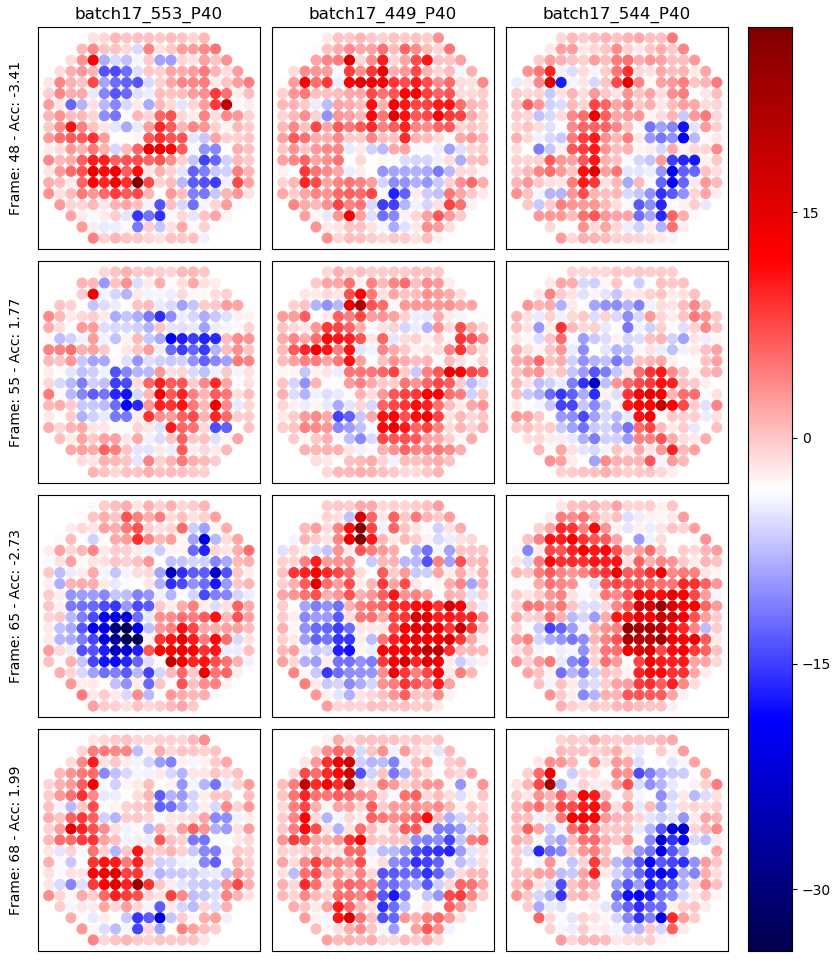
\includegraphics[scale=0.45]{Figures/results2.png}
	\caption{Comparing the Output of Three Cases Through Time: Sum of Channel Displacement in South-North Direction (mm). Three cases have been chosen at random from the data-set, corresponding to each of the three columns in this Figure. Each row corresponds to a time index of the earthquake (see the vertical markers in Figure~\ref{fig:earthquake}). The time frame is listed, as well as the earthquake acceleration at that time. The images are a graphical representation of the displacement value for each interstitial channel. Note that values are in the range $ \pm 30 $ i.e. the overall movement of that channel may be up to 30 mm in the south or north direction.}
	\label{fig:results2}
\end{figure*}

\noindent
For an alternative view on the previously illustrated example cases, the sum of level-by-level displacement can be seen in Figures~\ref{fig:levels1} and \ref{fig:levels2}. Similar to the top down view equivalent, Figure~\ref{fig:levels1} (west east displacement) shows little variation across the three sample cases for frames 65 and 68, with slightly more variation on a similar pattern seen in frames 48 and 55. Variations between cases for south-north displacement (Figure~\ref{fig:levels2}) for all four frames.
\\

\begin{figure*}[p]
	\centering
	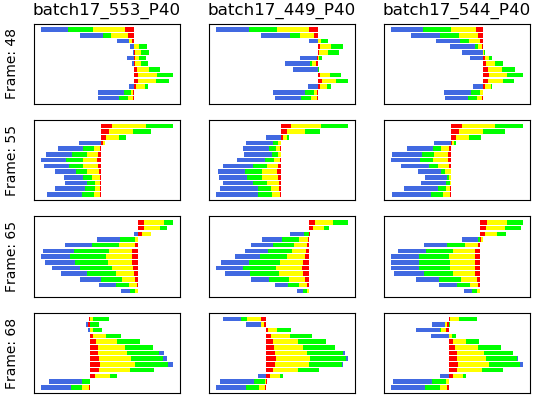
\includegraphics[scale=0.6]{Figures/level_results1.png}
	\caption{Comparing Output of Three Cases Through Time: Sum of Level Displacement in West-East Direction (mm). Three cases have been chosen at random from the data-set, corresponding to each of the three columns in this Figure. Each row corresponds to a time index of the earthquake (see the vertical markers in Figure~\ref{fig:earthquake}). The time frame is listed. The images are a graphical representation of the displacement value for each interstitial level.}
	\label{fig:levels1}
\end{figure*}

\begin{figure*}[p]
	\centering
	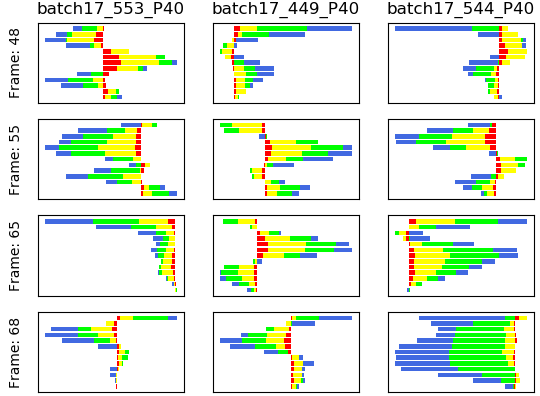
\includegraphics[scale=0.6]{Figures/level_results2.png}
	\caption{Comparing Output of Three Cases Through Time: Sum of Level Displacement in South-North Direction (mm). Three cases have been chosen at random from the data-set, corresponding to each of the three columns in this Figure. Each row corresponds to a time index of the earthquake (see the vertical markers in Figure~\ref{fig:earthquake}). The time frame is listed. The images are a graphical representation of the displacement value for each interstitial level.}
	\label{fig:levels2}
\end{figure*}


\subsubsection{Entire Data-set}


Several visualisations were generated based on the entire data-set of approximately 6500 samples. For the time frames highlighted in the previous section, Figures~\ref{fig:histo1} and \ref{fig:histo2} show histograms of all Parmec displacements outputs across all data-set samples. Note that for both displacement directions, the data at each time frame fits a symmetric bell curve distribution. 
\\

\noindent
For a single time frame (48) Figure~\ref{fig:composite} shows a channel by channel summation of the Parmec results across the entire data-set. This allows us to make comparisons between core regions. The outer channels tend to have negative (eastward) displacement, indicated in blue. As we move closer to the centre of the core, the displacement moves towards zero, indicated in white. Moving further towards the centre of the core, the displacement becomes increasingly positive (westward), indicated in red. The displacement values have strong radial symmetry about the centre. The uniform structure of the Parmec outputs in the aforementioned figure are interesting when considering that the input crack patterns are randomly generated.  
\\


\begin{figure*}[p]
	\centering
	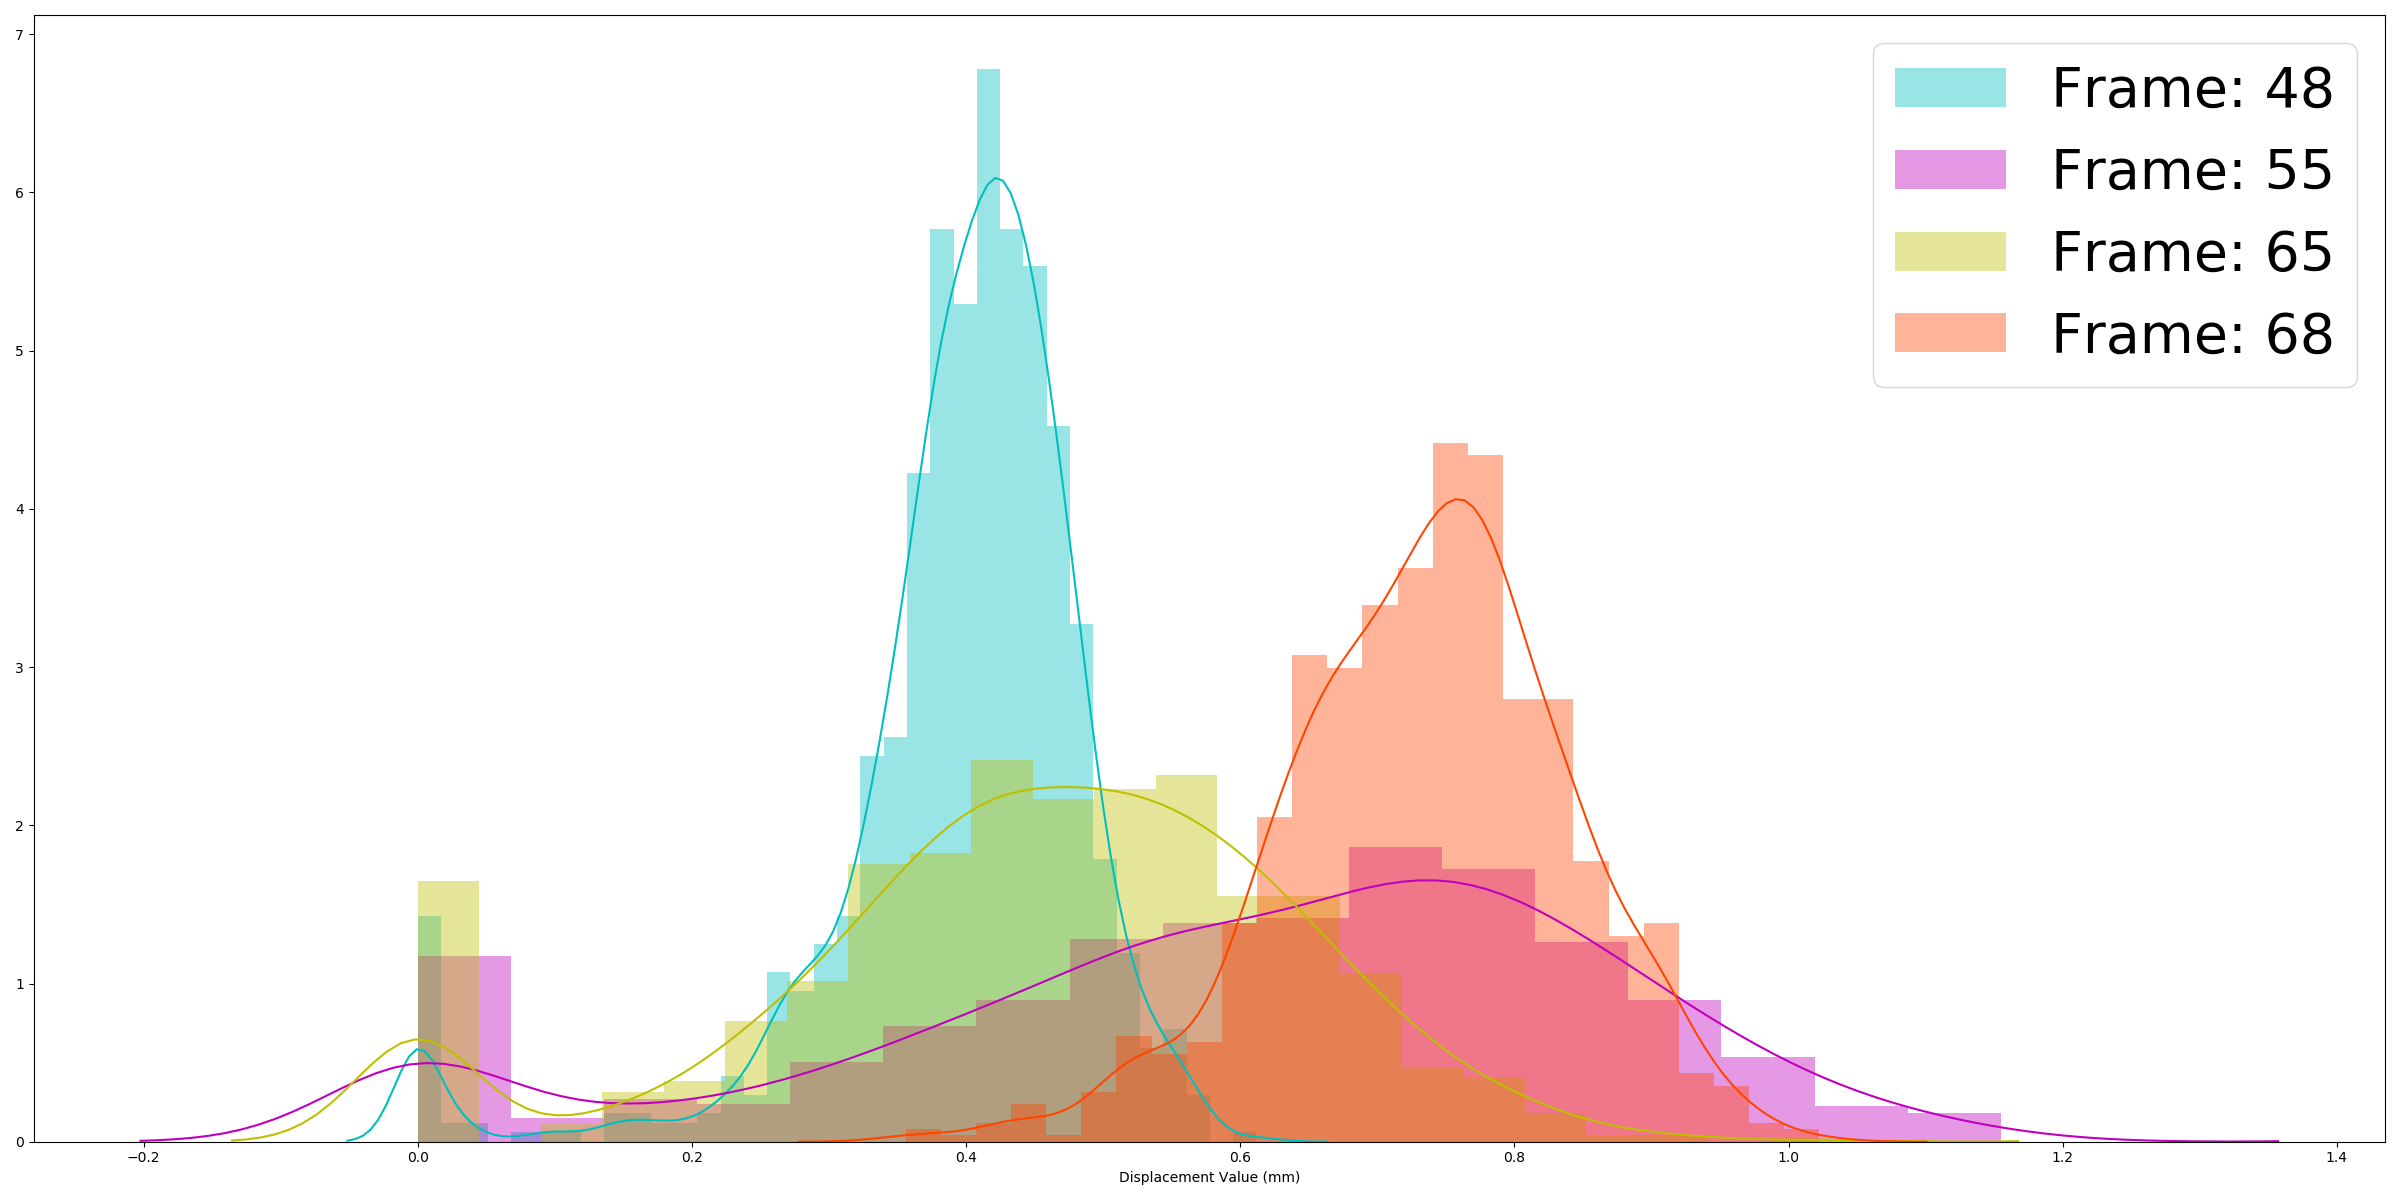
\includegraphics[scale=0.15]{Figures/histo1.png}
	\caption{Histogram of Sum Displacement of All Instances: West-East directional displacement. This plot shows a histogram for results across the data-set. The results for each time frame are Gaussian in shape i.e. a symmetric bell curve around a mean value. However, there seems to be a smaller peak near the left tail.}
	\label{fig:histo1}
\end{figure*}

\begin{figure*}[p]
	\centering
	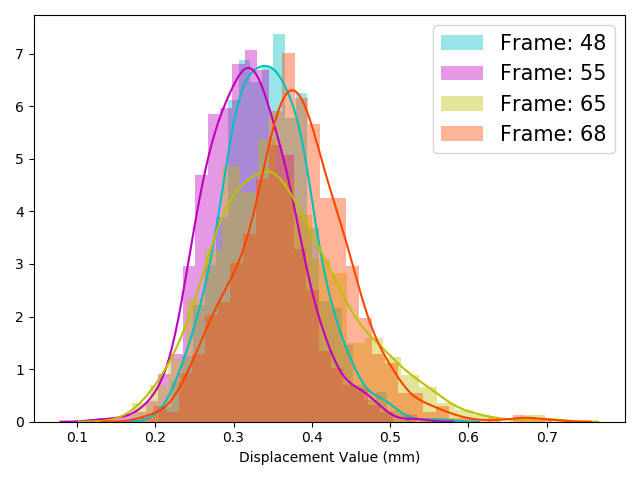
\includegraphics[scale=0.5]{Figures/histo2.png}
	\caption{Histogram of Sum Displacement of All Instances: South-North directional displacement. This plot is very similar to Figure~\ref{fig:histo1}. A Gaussian distribution can be seen similarly to the previous plot.}
	\label{fig:histo2}
\end{figure*}

\begin{figure}[ht]
	\centering
	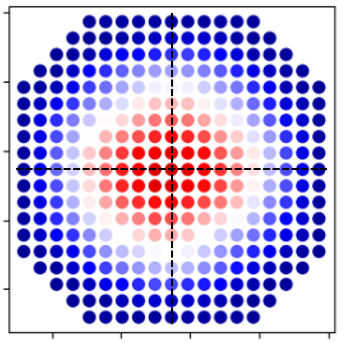
\includegraphics[scale=0.85]{Figures/compositeLines.png}
	\caption{Channel Summation for Time Frame 48: For each channel, the Parmec Outputs in the west-east direction were summed.}
	\label{fig:composite}
\end{figure}

\subsection{Output Correlation Analysis}

\noindent A natural question at this point would be: how do the individual label values from \ref{instance_result_matrix} correlate with each other? For example, do the results for central channels increase when those for outer channels increase? Or is the opposite the case, or neither? \\

\noindent Consider again Figure~\ref{fig:inter_order} which numbers each of the interstitial channels. Note that channels are numbered in rows from left to right and hence numerically close channels are not always physically close - e.g. 75 and 76, which are on opposite ends of the core. Using the numbers from Figure~\ref{fig:inter_order}, consider Figure~\ref{fig:channel_correlations}. It appears that channels which are physically close correlate strongly, with this tendency breaking down the further a two channels are away from each other. This would suggest it may be difficult to train a model capable of making accurate predictions across the whole core.
\\

\begin{figure}[h]
	\centering
	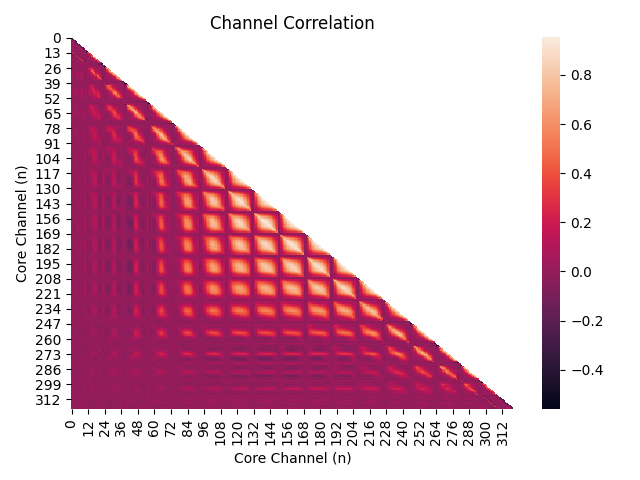
\includegraphics[scale=0.75]{Figures/channels_correlation.png}
	\caption{Correlation of Channel Results Against Each Other}
	\label{fig:channel_correlations}
\end{figure}

\begin{figure}[h]
	\centering
	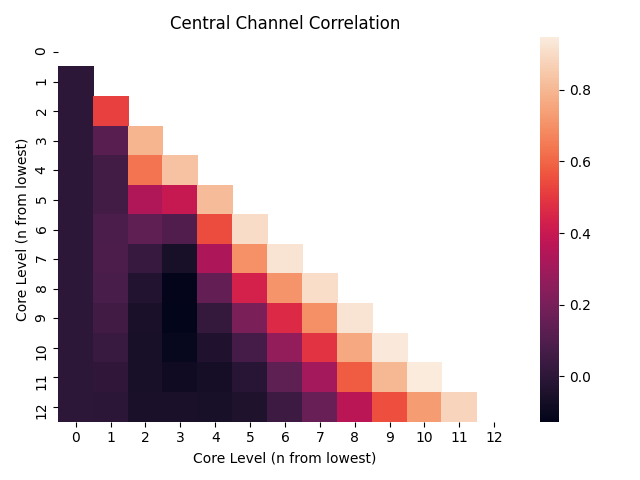
\includegraphics[scale=0.75]{Figures/central_channel_correlation.png}
	\caption{Correlation of Bricks of the Central Channel (161) Results Against Each Other}
	\label{fig:central_correlations}
\end{figure}


\noindent
Looking closely at only the correlations between results for the central interstitial channel (number 161 - see Figure~\ref{fig:inter_order}), we can again see a stronger correlation the closer two bricks are physically located (Figure~\ref{fig:central_correlations}).